\begin{figure*}[t]
  \centering
  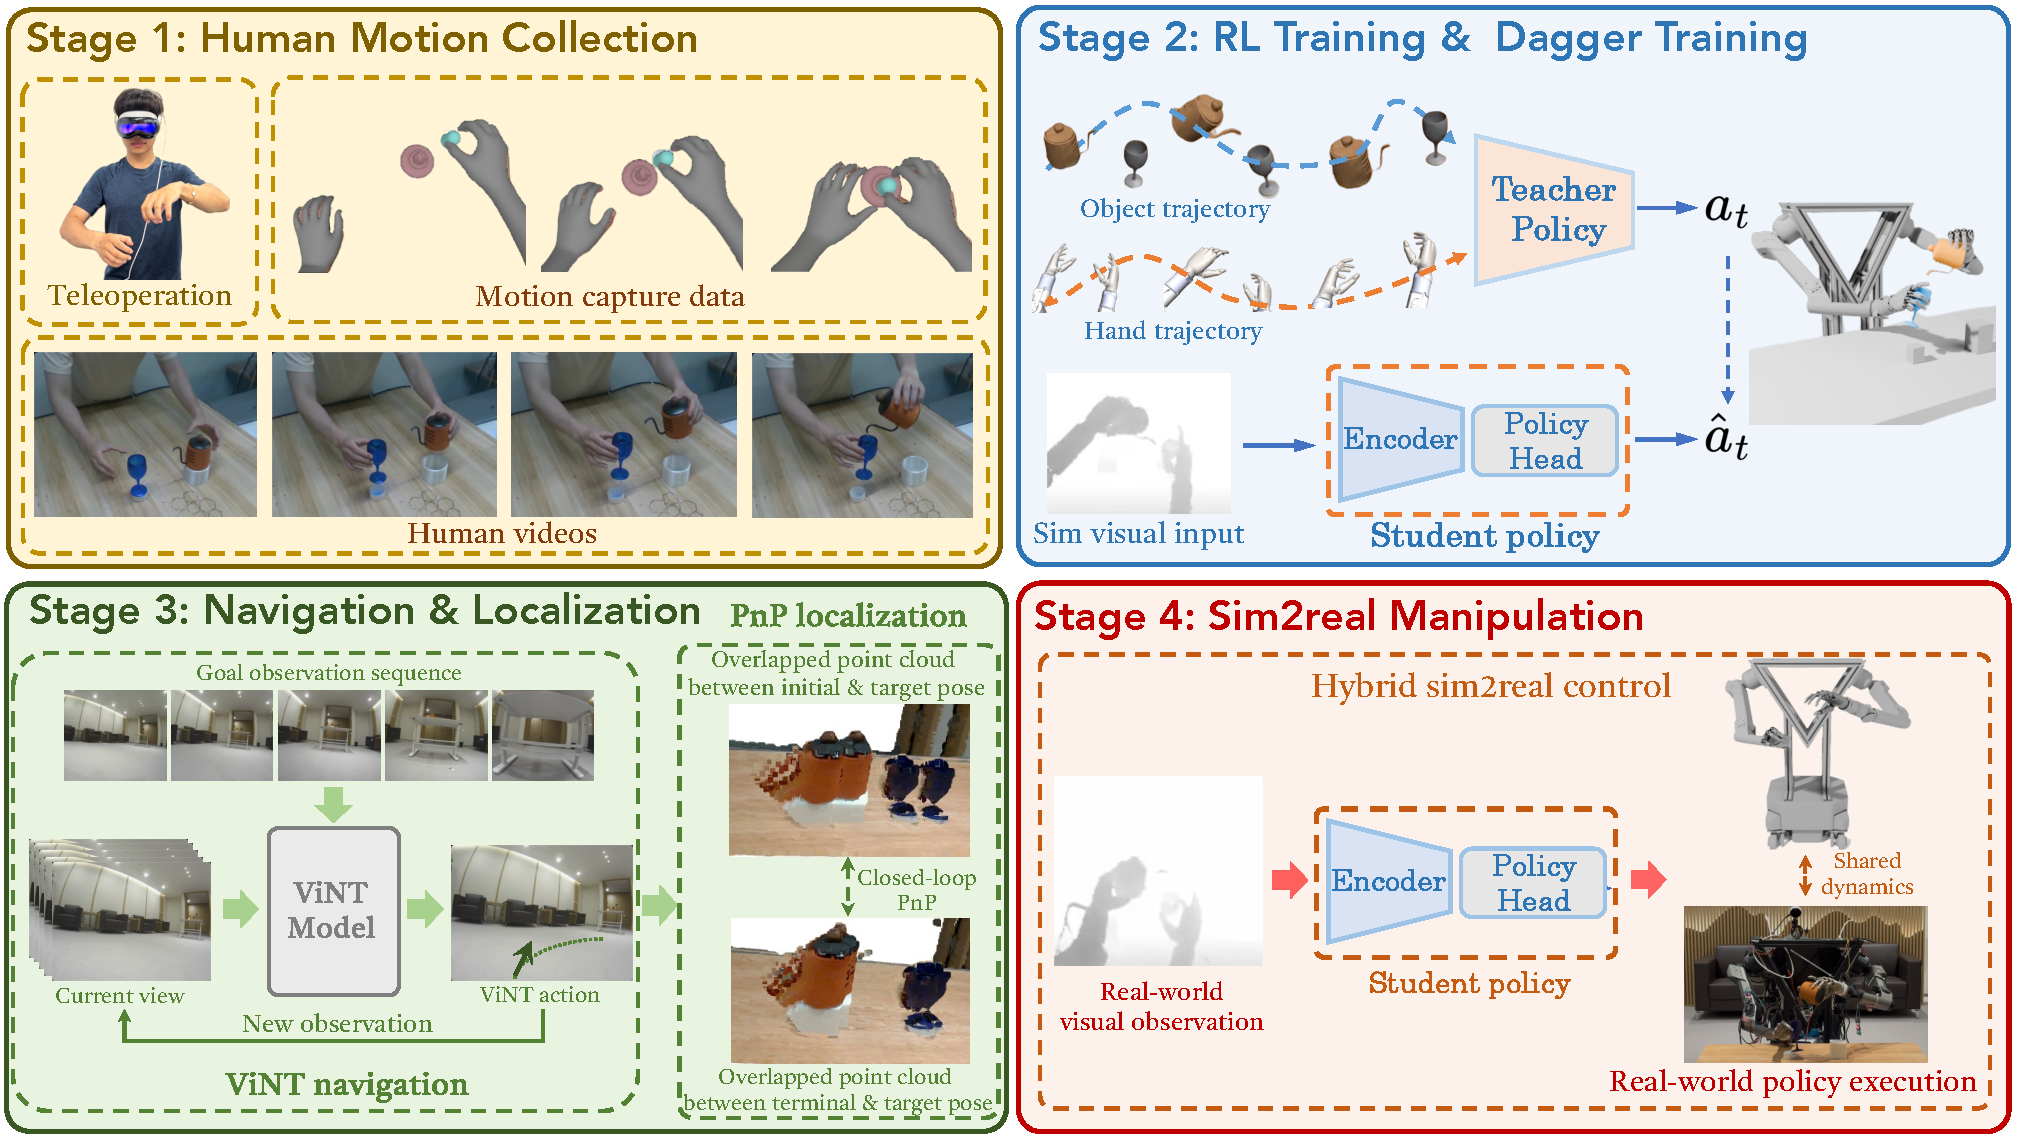
\includegraphics[width=1.0\linewidth]{figures/method_pic.pdf}
  \vspace{-15pt}
  \caption{ \textbf{The main pipeline of \ourshort.} \ourshort comprises a four-stage pipeline for achieving mobile bimanual dexterous manipulation through sim2real transfer. First, we acquire a one‑shot human demonstration drawn from diverse sources. Then, in stage 2, we train a state-based RL teacher policy, then apply DAgger to distill it into a vision‑based student policy. Following this, \ourshort execute long‑horizon navigation using ViNT, followed by closed-loop PnP to finely adjust the robot’s pose and achieve precise alignment in stage 3. Once localization is achieved, the student policy is deployed in a zero‑shot fashion directly in the real world.}
\label{fig:method}
\end{figure*}
\section{Reinforcement Learning Method}
\subsection{Task Formulation}
We define each task under the framework of goal-conditioned reinforcement learning. Our goal is to enable the robot to acquire the capability to convert the desired kinematic motion trajectory into physically executable robot behaviors. The tasks are formulated as the Markov Decision
Process~(MDP) $\mathcal{M}=(\mathcal{S}, \mathcal{A}, \mathcal{T}, \mathcal{R}, \gamma, \mathcal{G}$) , where $\mathcal{S}$ is the state space, $\mathcal{A}$ is the action space, $\mathcal{T}$ is the transition function, $\mathcal{R}$ is the reward, $\gamma$ is the discount factor, $\mathcal{G}$ is the reference trajectory. For goal-conditioned reinforcement learning,  the state $s \in \mathcal{S}$  includes the proprioception information $s^{p}$ and the goal state $s^{g}$ from $\mathcal{G}$, and the reward function at timestep $t$ is defined as $r_{t}=\mathcal{R}(s^{p}_{t}, s^{g}_{t})$. Under such a formulation, the policy is able to acquire complex and fine-grained behaviors from diverse reference trajectories without relying on labor-intensive reward engineering. 


\subsection{Collect One-shot Human Motion}
To validate the effectiveness and robustness of \ourshort, we employ three distinct sources of human motion: teleoperation in simulation, motion capture data obtained from public datasets, and hand-object poses extracted from raw videos. Moreover, by leveraging merely a single human reference trajectory in conjunction with RL training, we are able to derive the generalizable robot policy without the need for collecting extensive demonstrations.

\textbf{Teleoperation in simulation:} We provide access to the pre-configured simulation that enables direct teleoperation of the robot for collecting demonstrations. The Apple Vision Pro is utilized to extract hand poses and arm movements, with data captured at a frequency of 75 Hz.

\textbf{Mocap data:} In contrast to direct teleoperation in simulation, retargeting mocap data to robotic hands presents significant challenges due to the embodiment gap between human and robotic hand structures. This discrepancy renders the retargeted trajectories from mocap data unsuitable for direct replay in simulation. Consequently, RL is often employed to enable robots to learn the desired behaviors from reference trajectories. In our study, we acuqire human motion capture data from the OakInk2~\cite{zhan2024oakink2} dataset. 

\begin{figure}[h]
  \centering
  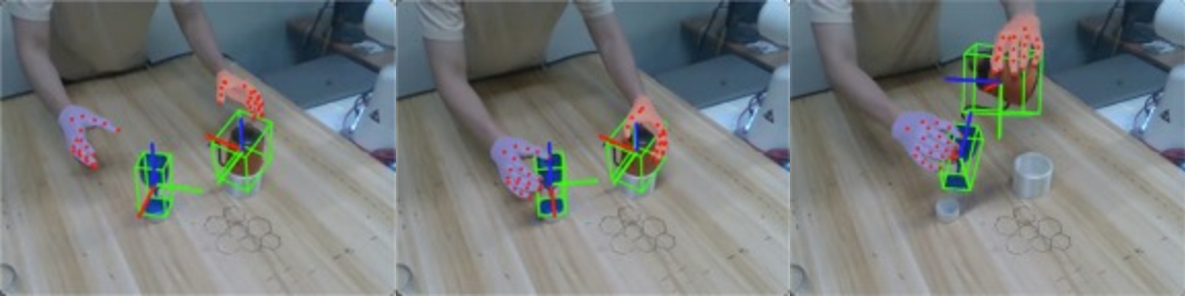
\includegraphics[width=1.0\linewidth]{figures/foundationpose_pic.pdf}
  \vspace{-15pt}
  \caption{\textbf{Pose extraction from videos.} We utilize FoundationPose to extract the pose trajectories of multiple objects and employ WiLoR to capture the poses of both hands along with the positions of their finger joints.}
  \label{fig:fp}
\end{figure}
\begin{figure}[h]
  \centering
  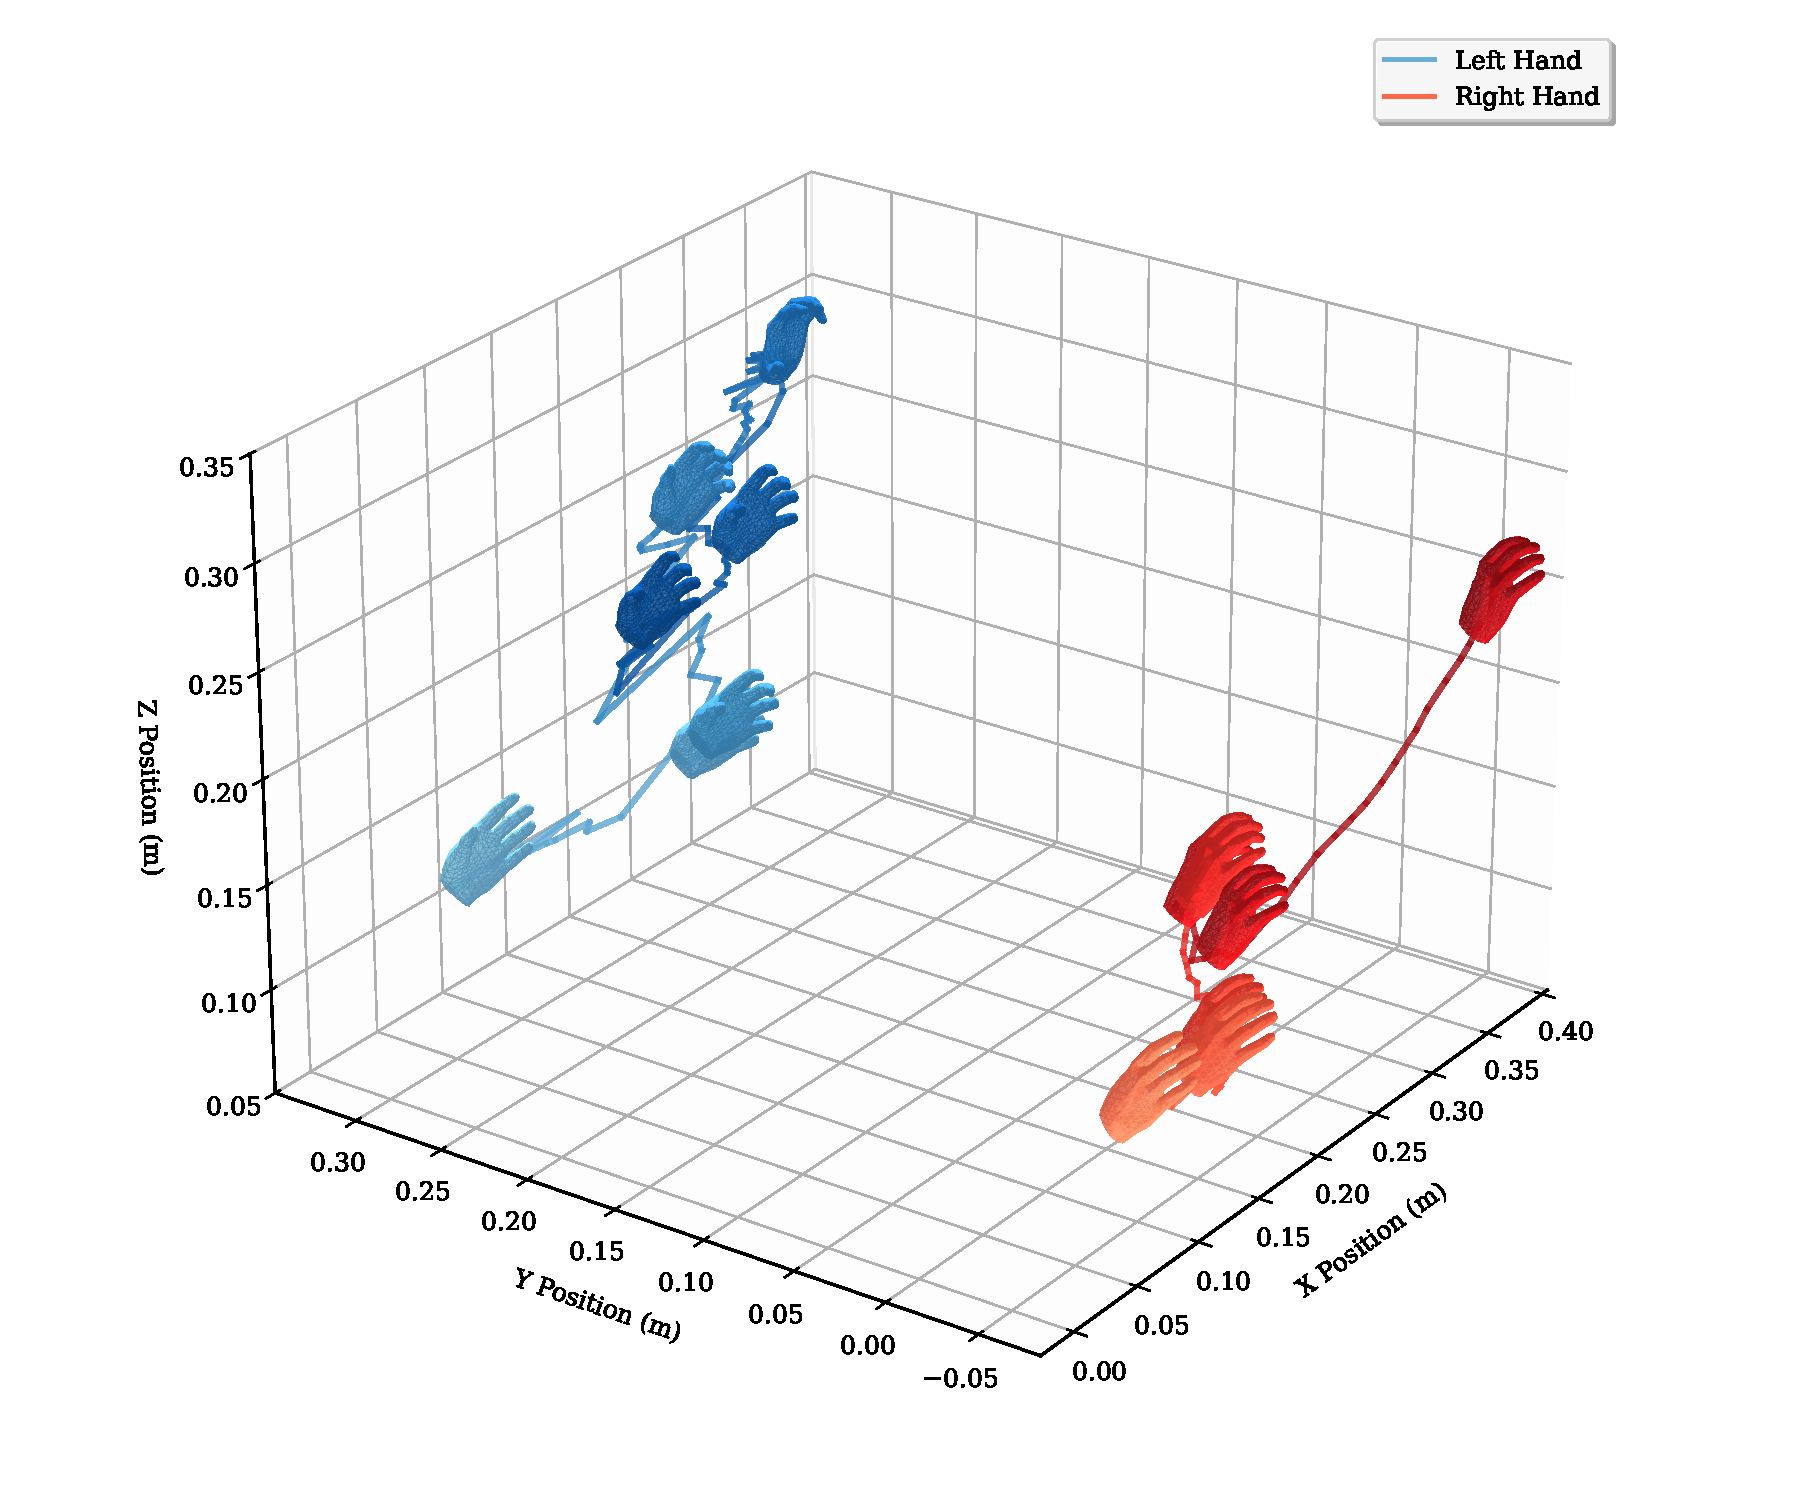
\includegraphics[width=1.0\linewidth]{figures/hand_traj_pic.pdf}
  \vspace{-15pt}
  \caption{ \textbf{The visualization of hand motion trajectory.} We utilize WiLoR along with a PnP algorithm to precisely transform the estimated hand poses into the robot’s frame.}
  \label{fig:handtraj}
\end{figure}
\textbf{Extracted arm and hand poses from videos:} 
Leveraging video data holds considerable promise for unlocking vast quantities of information to facilitate robot learning. To this end, we also provide a pipeline for extracting human hand poses and object trajectories directly from raw video. To acquire the hand poses, we first employ WiLoR~\cite{potamias2024wilor} to detect the hands in each video frame and extract 2D hand keypoints along with their corresponding 3D counterparts. We then select a relatively stable subset of keypoints for the subsequent estimation, specifically those located at the wrist and the metacarpophalangeal joints. The spatial translation of the wrist in the camera coordinate system is estimated by solving a Perspective-n-Point~(PnP) problem~\cite{li2012robust} based on the 2D-3D correspondences, while the palm's orientation is derived by fitting a plane to the selected 3D keypoints. The extraction results are shown in Figure~\ref{fig:handtraj}. Regarding the manipulated objects, we employ FoundationPose~\cite{wen2024foundationpose} to estimate the object poses directly from video frames, and utilize ARCode~\cite{arcode2022} scanning to reconstruct the object mesh. By leveraging the aforementioned procedures, we can align the hand and object poses extracted from the video with the robot's frame to facilitate the subsequent learning process.   

\textbf{Synthesize multiple trajectories:} To obtain a more generalizable policy, we perform the trajectory augmentation for the one-shot human motion reference by randomizing positions and orientations of the objects in a predefined range. The hand and object poses across the augmented trajectories are transformed as follows:
\begin{equation}
\hat{\mathbf{A}}^{\mathrm{pose}}\left[\tau_k\right]=\mathbf{T}^{\mathrm{trans}} \cdot\mathbf{A}^{\mathrm{pose}}\left[\tau_k\right] .
\end{equation}
For any given frame $k$ in the trajectory $\tau$, we apply a transformation matrix $\mathbf{T}^{\mathrm{trans}}$ to alter its pose, where $\mathbf{A}^{\mathrm{pose}}$ may represent either the object pose or the hand pose. By editing the reference trajectory, we enable spatial generalization from a single human motion demonstration, obviating the need to manually collect large numbers of teleoped demonstrations.

Upon obtaining synthesized object and hand trajectories from various data sources, we initially employ DexPilot~\cite{handa2020dexpilot}, a popular retargeting method to map the captured human hand poses onto corresponding robot hand configurations. Subsequently, reinforcement learning is leveraged to refine and adapt the initialized robot behaviors.



\subsection{Generalizable Reward Design for Manipulation}
Standard reinforcement learning typically relies on hand-crafted reward functions tailored to each specific task. However, designing such complicated reward structures often impedes scalability and usability, particularly for the dexterous hand. To alleviate this issue, we leverage one-shot human demonstration combined with a generalizable reward formulation so that one unified reward function can be reused across tasks and simplify the specific design of challenging, long-horizon manipulation tasks. Recent advancements in locomotion~\cite{luo2023perpetual,peng2018deepmimic,he2025asap,allshire2025visual} have predominantly adopted such design paradigms for training humanoid or quadruped robots. However, manipulation tasks introduce additional complexities, as robots must not only perceive their own proprioception states but also effectively interact with external objects. Therefore, we propose a generalizable reward framework tailored for manipulation tasks, capable of being applied across diverse tasks. 

Specifically, we design the following three reward terms:

\begin{figure}[t]
  \centering
  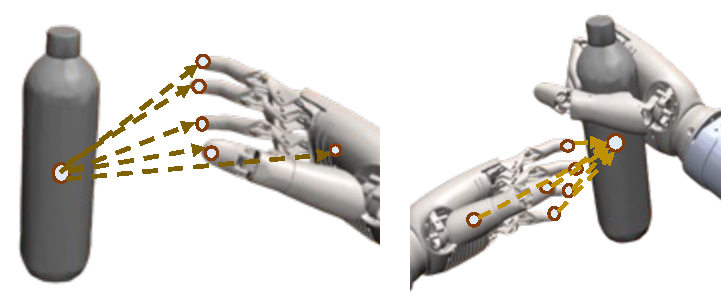
\includegraphics[width=1.0\linewidth]{figures/distance-chain_pic.pdf}
  \vspace{-15pt}
  \caption{ \textbf{Object-centric distance chain.} This reward term is computed by tracking the temporal variations of vectors formed between the object center and each fingertip as well as the palm of both hands.}
  \label{fig:distance-chain}
\end{figure}
\textbf{Object-centric distance chain:}  
Capturing the dynamic spatial relationships between the human hands and the object stands as a pivotal factor in enabling the policy to acquire fine-grained hand-object interaction skills. As illustrated in Figure~\ref{fig:distance-chain}, we designate the coordinates of the fingertips and palm of the hand, along with  the center of the object's collision mesh, as keypoints. By modeling the temporal variation of vectors between these keypoints, we formulate the following reward function:
% \begin{equation}
%     r_{chain} = \frac{1}{n}\sum_{i=1}^n\left\|\boldsymbol{\vec{r}}_{re f}^{(i)}-\boldsymbol{\vec{r}}^{(i)}\right\|
% \end{equation}

\begin{equation}
r_{\text{chain}} =
\begin{cases}
\exp\left\{- \frac{1}{n} \sum_{i=1}^n \left\| \vec{r}_{\text{ref}}^{(i)} - \vec{r}^{(i)} \right\| \right\}, & \text{if } N_{\text{contact}} \geq N_{\text{num}} \\
0, & \text{otherwise},
\end{cases}
\end{equation}


where ${\vec{r}}^{(i)}$ is the vector from object center to the fingertip or palm. Furthermore, we incorporate contact information into this reward term.  Specifically, during the computation of the distance chain, we also evaluate the number of contact points between the fingertips and palms of both hand mesh $\mathbf{C}_{\text{hand}}$ and the object's collision mesh $\mathbf{C}_{\text{obj}}$. This reward component is activated only when the number of contact points $N_{\text{contact}}$ exceeds a predefined threshold $N_{\text{num}}$, ensuring that the policy attends to physically meaningful hand-object interactions.
\begin{equation}
    N_{\text{contact}} = \frac{1}{2}\sum_{j}\sum_i \mathbbm{1}(\mathbf{C}_{\text{hand}}^{i}, \mathbf{C}_{\text{obj}}^{j}),
\end{equation}






where $\mathbbm{1}(\cdot, \cdot)$ is the indicator function that evaluates whether a collision occurs between the hand and the object. In addition, we also encourage the robot to favor joint positions in the retargeted trajectories during exploration. 



\textbf{Object trajectory tracking:}
For manipulation tasks which adopt human motion, a critical indicator of policy success lies in its ability to track and follow the desired object trajectory. To this end, we introduce an additional reward component that explicitly aligns the policy’s behavior with the target object’s trajectory:

\begin{equation}
r_{\text{obj}} = \exp\left(-k_1 \cdot \left\| \mathbf{p}_{\text{obj}} - \mathbf{p}_{\text{ref}} \right\|^2 - k_2 \cdot \left( d_{\text{quat}}(\mathbf{q}_{\text{obj}}, \mathbf{q}_{\text{
ref
}}) \right)^2\right)
\end{equation}

where $k_{1}$, $k_{2}$ are the coefficients corresponding to the position and orientation terms in the $r_{\text{obj}}$.  $\mathbf{p}_{\text{obj}}$ and $\mathbf{q}_{\text{obj}}$ represent the current position and orientation of the object, while $\mathbf{p}_{\text{ref}}$ and $\mathbf{q}_{\text{ref}}$ denote the position and orientation along the reference trajectory. The term $d_{\text{quat}}$ measures the distance between two quaternions.


\textbf{Power penalty:} In order to enhance the smoothness of policy execution, we design a power penalty reward to alleviate the jittering actions:

\begin{equation}
r_{\text{penalty}} = -\lambda \sum_{j \in \mathcal{J}_{\text{hand}}} \left| f_j \cdot \dot{q}_j \right|,
\end{equation}

where $\lambda$ is the coefficient of $r_{\text{penalty}}$. $\mathcal{J}_{\text{hand}}$ denotes the set of all hand joints. $f_{j}$ is the actuation force applied at joint $j$, and $\dot{q}_j$ is the velocity of joint $j$. 


By integrating all these reward components, the policy is endowed with the capacity to tackle a wide spectrum of challenging and diverse manipulation tasks.


\subsection{Residual Action Learning}
 While human trajectories provide coarse guidance on arm and hand movements throughout task execution, they often lack the precision required for accurate object interactions. To address this, we design distinct learning strategies for the arm and hand. For the arm, we decompose actions into coarse and fine components. At each timestep $t$,  the coarse action $\boldsymbol{a_{g}}$ is directly derived from the human trajectory, offering a general movement direction. The fine component $\Delta_{\boldsymbol{a_{f}}}$ is predicted by a learned network $\Delta_{\boldsymbol{a_{f}}}=\boldsymbol{\pi(s)}$, refining the motion to ensure precise control. Hence, the final form of arm action $\boldsymbol{a_{arm}}$ is $\boldsymbol{a_{arm}}=\Delta_{\boldsymbol{a_{f}}}+\boldsymbol{a_{g}}$. Regarding the hand part, due to inaccuracies in retargeting human demonstrations, we entirely adopt the network output $\boldsymbol{a_{hand}}$  to model the interaction behaviors with objects. This hybrid approach allows the policy to capture the overarching structure of human motion while learning the nuanced adjustments necessary for effective and precise manipulation for robots. 

In addition, given the high-dimensional action space and inherent complexity of bimanual dexterous hand tasks, we incorporate the early termination strategy to curtail inefficient exploration~\cite{peng2018deepmimic}. Meanwhile, to enable the acquisition of an initial viable behavior, we disable object collisions during the early stages of training, allowing the policy to first focus on learning the approximate motion trajectory.


\subsection{Reinforcement Learning Algorithm}
We implement two distinct reinforcement learning algorithms. DrM~\cite{xudrm}, an off-policy method, leverages a dormant ratio mechanism~\cite{sokar2023dormant} to enhance exploration capabilities and demonstrates high sample efficiency. We adapt the network architecture and take the state observation as inputs for state-based RL training. DrM training for all tasks is conducted in the MuJoCo simulation environment. Concurrently, we also instantiate the tasks in the MJX platform, which supports GPU-accelerated parallel training, and employ the PPO algorithm to significantly reduce the overall wall-clock training time. More details can be found in Appendix~\ref{sec:state-rl}. 




